\section{Contrast and Multiple Testing}

\subsection{Contrast}

The $F$-test is rather unspecific and gives us basically a yes/no answer. It does not tell us what treatment (or combination of treatments) is significant. Such kind of questions can be formulated as so-called \textbf{contrasts}. As hypothesis we choose:
$$H_0 : \sum_{i=1}^g c_i \mu_i = 0 \text{ and } H_A : \sum_{i=1}^g c_i \mu_i \neq 0$$

Typically we have the side constraint that $\sum_{i=1}^g c_i = 0$. The contrast is about the differences between treatments and not about the overall response. We estimate the value of $\sum_{i=1}^g c_i \mu_i$ with:
$$\sum_{i=1}^g c_i \hat \mu_i = \sum_{i=1}^g c_i \bar y_{i.}$$

In addition, we could derive its accuracy (standard error), construct confidence intervals and do tests.

\begin{lstlisting}
library(multcomp)
## linfct is our contrast
fit.glht <- glht(fit, linfct = mcp(group = c(1, -1/2, -1/2)))
summary(fit.glht)
\end{lstlisting}

Every contrast has an associated sum of squares:
$$SS_C = \frac{(\sum_{i=1}^g c_i \bar y_{i.})^2}{\sum_{i=1}^g \frac{c_i^2}{n_i}}$$	

It has one degree of freedom and therefore $MS_C = SS_C$. We have:
$$\frac{MS_C}{MS_E} \sim F_{1, N-g}$$

Two contrasts $c, c^*$ are orthogonal if:
$$\sum_{i=1}^g \frac{c_i c_i^*}{n_i} = 0$$

In this case, the corresponding estimates are independent. If we have $g$ treatments, we can find
$g - 1$ different orthogonal contrasts (one dimension is already used by the global mean). A set of orthogonal contrasts partitions the treatment sum of squares meaning that if
$c^1, ..., c^{g-1}$ are orthogonal contrasts it holds that:
$$SS_{c^1} + ... + SS_{c^{g-1}} = SS_{Trt}$$

Multiple contrasts are all orthogonal if and only if for the matrix $C$ that represents them, $C^\top C$ is diagonal.


\subsection{Multiple Testing}

The problem with all statistical tests is the fact that the overall type I error rate increases with increasing number of tests. This means that if we perform many tests, we expect to find some significant results, even if all $H_0$ are true. Somehow we have to take into account the number of tests that we perform to control the overall type I error rate. \medskip

We list the potential outcomes of a total of $m$ tests, among which $m_0$ $H_0$ are true:
\begin{center}
	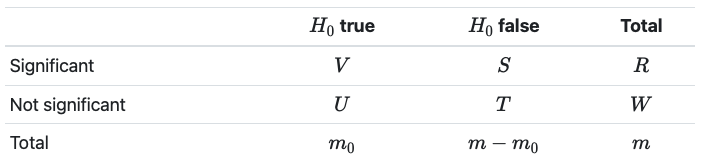
\includegraphics[width=\linewidth]{multiple_testing.png}
\end{center}

For example, $V$ is the number of wrongly rejected $H_0$ (type I errors, also known as FP). Using this notation, the overall or family-wise error rate (FWER) is defined as the probability of rejecting at least one of the true $H_0$'s:
$$\text{FWER} = P(V \geq 1)$$

The family-wise error rate is very strict in the sense that we are just interested in whether there is at least one wrong rejection. We say that a procedure controls the family-wise error rate in the strong sense at level $\alpha$ if FWER $\leq \alpha$ for any configuration of true and non-true $H_0$'s. \medskip

Another error rate is the FDR which is the expected fraction of false discoveries:
$$\text{FDR} = E \left[ \frac{V}{R} \right]$$

Controlling FDR at level $0.2$ means that on average in our list of significant findings only $20\%$ are false positives. If a procedure controls FWER at level $\alpha$, FDR is automatically controlled at level $\alpha$ too. This does not hold the other way around. \medskip

We can also control the error rates for confidence intervals. We call a set of confidence intervals simultaneous confidence intervals at level $(1 - \alpha)$ if the probability that all intervals cover the corresponding true parameter value is $(1 - \alpha)$. This means that we can look at all confidence intervals at the same time and get the correct “big picture” with probability $(1 - \alpha)$. \medskip

In the following, we typically start with individual p-values (the ordinary p-values corresponding to the $H_{0,j}$'s) and modify them such that the appropriate overall error rate (like FWER) is being controlled. The modified p-values should be interpreted as the smallest overall error rate such that we can reject the corresponding null hypothesis.

\subsubsection{Bonferroni}

The Bonferroni correction is a very generic but conservative approach. The idea is to use a more restrictive (individual) significance level of $\alpha^* = \alpha / m$. This procedure controls the FWER in the strong sense for any dependency structure of the different tests. Especially for large $m$, the Bonferroni correction is very conservative leading to low power.

\begin{lstlisting}
library(multcomp)
## K is a matrix with each row being a contrast
fit.glht = glht(fit, linfct = mcp(group = K))
summary(fit.glht, test = adjusted("bonferroni"))
\end{lstlisting}

\subsubsection{Bonferroni-Holm}

The Bonferroni-Holm procedure also controls the FWER in the strong sense. It is less conservative and uniformly more powerful, which means always better, than Bonferroni. It works in the following sequential way:
\begin{enumerate}
	\item Sort $p$-values from small to large
	\item For $j = 1,...$: Reject null hypothesis if $p_j \leq \frac{\alpha}{m-j+1}$
	\item Stop when reaching the first non-significant $p$-value and do not reject the remaining null hypotheses.
\end{enumerate}

Note that this procedure only works with p-values but cannot be used to construct confidence intervals.
\begin{lstlisting}
summary(fit.glht, test = adjusted("holm"))
\end{lstlisting}

\subsubsection{Scheffe}

The Scheffe procedure controls for the search over any possible contrast. This means we can try out as many contrasts as we like and still get honest p-values! This is even true for contrasts that are suggested by the data, which were not planned beforehand, but only after seeing some special structure in the data. The price for this is low power. \medskip

The Scheffe procedure works as follows: We start with the sum of squares of the contrast $SS_C$. Then we build the $F$-ratio:
$$\frac{SS_C/(g-1)}{MS_E}$$

\subsubsection{Tukey Honest Significant Differences}

A special case of a multiple testing problem is the comparison between all possible pairs of treatments. The output is a matrix of $p$-values of the corresponding comparisons. We could now use the Bonferroni correction method. However, there exists a better, more powerful alternative which is called Tukey Honest Significant Differences (HSD). \medskip

Think of a procedure that is custom tailored for the situation where we want to do a comparison between all possible pairs of treatments. We get both $p$-values (which are adjusted such that the family-wise error rate is being controlled) and simultaneous confidence intervals.
\begin{lstlisting}
TukeyHSD(fit)
\end{lstlisting}


\subsubsection{Multiple Comparisons with a Control}

 if we want to compare all treatment groups with a control group, we have a so-called multiple comparisons with a control (MCC) problem. The corresponding custom-tailored procedure is called Dunnett procedure. It controls the family-wise error rate in the strong sense and produces simultaneous confidence intervals. 
 
\begin{lstlisting}
fit.glht <- glht(fit, linfct = mcp(group = "Dunnett"))
summary(plant.glht)
\end{lstlisting}

 We get smaller $p$-values than with the Tukey HSD procedure because we have to correct for less tests; there are more comparisons between pairs than there are comparisons to the control treatment.
